\documentclass{article}
\usepackage[utf8]{inputenc}
\usepackage{geometry}
\usepackage{color}
\usepackage{hyperref}   % use for hypertext links, including those to external documents and URLs
\usepackage{natbib}
\usepackage{graphicx}

\geometry{hmargin=3cm,vmargin=3cm}

\title{\vspace{\fill} Bilan sur le déroulement du projet GL \vspace{\fill}}

\author{Équipe 17 \\\\ Anaïs Hadj-Azzem - Lucas Grellier - Théo Caché - Clément Vanhemelryck - César Dumas}

\date{\\}

\hypersetup{
  colorlinks=true,
  linkcolor=blue,
  urlcolor=red,
  linktoc=all
}
% don't need the following. simply use defaults
\setlength{\baselineskip}{16.0pt}    % 16 pt usual spacing between lines

\setlength{\parskip}{3pt plus 2pt}
\setlength{\parindent}{20pt}
\setlength{\oddsidemargin}{1cm}
\setlength{\evensidemargin}{1cm}
\setlength{\marginparsep}{0.75cm}
\setlength{\marginparwidth}{2.5cm}
\setlength{\marginparpush}{1.0cm}
\setlength{\textwidth}{150mm}
\renewcommand{\contentsname}{Table des matières}

\begin{document}

\maketitle
\thispagestyle{empty}
\setcounter{page}{0}
\newpage

\tableofcontents
\thispagestyle{empty}
\setcounter{page}{0}
\newpage

\section{Description de l'organisation}
\subsection{Une journée en tant que membre de l'équipe 17}
Dès le début du projet, nous avons décidé d'instaurer certaines règles afin d'éviter tout conflit au sein de l'équipe, et ainsi mener ce projet dans de bonnes conditions. \newline
Tout d'abord, chaque membre de l'équipe était tenu d'arriver dans les locaux de l'ENSIMAG entre 8h et 10h, à l'exception d'un seul membre, chargé d'assister au cours magistral.
Selon l'intitulé de ce cours, nous choisissions ensemble la personne qui nous semblait être la plus apte à assister à ce cours, lors de la deuxième réunion de la journée,
dont le déroulement est décrit plus bas dans cette partie. \newline
Durant ce temps, les 4 autres membres effectuent la première réunion de la journée. Plusieurs points y sont évoqués :
\begin{itemize}
\item Les objectifs de chacun en terme technique pour la journée. Cela permet à chaque membre de l'équipe de connaître l'avancement du projet et ainsi procéder à des changements d'organisation si besoin.
\item Les éventuels problèmes rencontrés lors de la journée précédente, afin de savoir si certains ont des idées pour résoudre ces problèmes.
\item La répartition des tâches, par exemple savoir qui se charge de mettre à jour le planning, de rédiger les documents des suivis etc...
\item Les indisponibilités de chacun, afin de pouvoir organiser au mieux le déroulement de la journée.
\end{itemize}
Dès la fin du CM, un membre de l'équipe fait un "debrief" de la réunion à la personne manquante. \newline
Dans une ambiance sérieuse, concentrée et pleine d'entraide, les heures passent. Le repas de midi est aussi une bonne occasion d'aborder les problèmes ou réussites de la matinée. En fin d'après midi, quelques dizaines de minutes avant le départ du premier membre, la deuxième réunion
de la journée est effectuée. Cette fois-ci, l'intégralité de l'équipe est présente et nous y évoquons :
\begin{itemize}
\item Le travail effectué au cours de la journée. Le planner Réalisation est alors mis à jour.
\item Les problèmes rencontrés, s'ils ont été résolus ou non, et dans ce cas un brainstorming est effectué pour tenter de trouver une solution.
\item Ce que chacun a prévu de faire dans la journée suivante ou dans la fin de la journée. Une réorganisation des membres de l'équipe peut être discuté si
quelqu'un juge cela nécessaire.
\item Si un cours magistral est tenu le lendemain, nous choisissons la personne qui sera tenu d'y assister.
\end{itemize}
Les membres de l'équipe 17 travaillent le week-end ! Les salles informatiques de l'ENSIMAG n'étant pas toujours disponibles,
nous avons tout de même décidé de nous retrouver le week-end. Nous avons jugé important d'être le plus souvent ensemble pour travailler,
pour des raisons d'efficacité mais aussi car nos compétences et connaissances s'avèrent parfois être complémentaires. \newline
En résumé : les membres de l'équipe 17 passent dans l'ensemble une bonne journée, modulo le nombre de bugs à résoudre!

\subsection{La répartition des tâches}
En effectuant nos auto-évaluations lors de la préparation du premier suivi, nous avons réalisé que nous formions une équipe homogène sur le plan des capacités techniques et nous avons donc pu séparer les tâches en grande partie selon les préférences de chacun. Évidemment, les rôles affectés lors des premières séances n'ont pas été définitifs et ont été modulés au vu des besoins. \newline
Dans un premier temps, nous avions choisi la répartition des tâches suivante :
\begin{itemize}
\item Anais et Théo travaillaient sur le lexer. Une fois celui-ci terminé, nous avons jugé qu'une seule personne était nécessaire pour
mener à bien la fin de la partie A. Ainsi, Théo a commencé l'extension MATH, attiré par le côté mathématique de la tâche.
\item César et Clément.
\item Lucas été chargé, dans un premier temps, des tests : automatisation, homogénéisation etc... Puis nous avons remarqué qu’une personne assignée à
faire uniquement des tests était finalement une manière peu productive de fonctionner, certes intéressante mais pas suffisante. Ainsi, Lucas a rapidement commencé
à travailler sur la partie C, notamment sur les options et la compréhension des travaux à effectuer.

\end{itemize}
L'étape A ayant été fonctionnelle rapidement, Anais a commencé l'étape C, rejoint par Clément, chargé de finir les options. César a alors travaillé en autonomie
sur la partie avec objet l'étape B, déjà bien commencée lors de cette décision. Ces décisions ont été capitales à l'avancement du projet,
et nous réalisons qu'elles auraient pu être optimisées. En effet, nous aurions pu adopter les choix suivants :
\begin{itemize}
\item Ne pas commencer l'extension MATH si tôt :  ainsi, Théo aurait pu commencer la partie C avec Lucas, du moins pour la partie sans-objet. Puis
dès les premiers résultats satisfaisants, Théo aurait pu commencer l'extension.
\item Se concentrer sur la partie C sans option : 3 ressources auraient pu être mobilisées à la réalisation de la partie C. Lorsque
les grandes lignes auraient été traitées, nous aurions pu désigner quelqu'un pour effectuer les options.

\end{itemize}
Dans l'ensemble, nous sommes tous d'accord pour dire qu'il aurait fallu accorder plus de temps et de ressources à cette partie, qui
demandait beaucoup de travail.

En outre, chaque membre de l'équipe a participé à l'étape de validation sur les différentes parties : des tests \textit{white-box }et \textit{black-box} ont
donc été effectués. Nous réalisons ainsi l'importance des tests \textit{white-box}, qui nous ont permis de déceler certaines erreurs.

\subsection{La répartition des rôles}
Lors de la première semaine de ce projet, du fait de l'homogénéité de nos compétences,
personnes n'avaient de rôle clairement défini. Cependant, nous avons très vite pris conscience de l'importance et de la nécessité de
définir des rôles, dans un soucis d'efficacité.
Ainsi, les rôles attribués lors de ce projet sont :
\begin{itemize}
\item Lucas, \textbf{responsable des tests} : automatisation, homogénéisation, vérification des tests. Par vérification, nous entendons la vérification du
bon fonctionnement du compilateur sur celui-ci, la qualité du test, et sa position dans l'arborescence des répertoires du dossier ProgetGL.
\item César, \textbf{risk manager} : revient sur les décisions prises lors des réunions, et s'assure que ces dernières sont les plus optimales
en termes techniques et organisationnelles.
\item Anais, \textbf{responsable communication} :  mise à jour du planning, et rappel au reste de l’équipe des dates butoirs à respecter.
\item Théo, \textbf{responsable de l'extension} : gestion entière de l'extension.
\item Clément, \textbf{chef de projet} : intervient dans différentes situations. Il anime notamment les deux réunions quotidiennes et prend la décision finale en cas de désaccord entre plusieurs membres de l'équipe.
\end{itemize}
Une fois ces rôles définis, nous avons fait preuve de bien plus d'efficacité : nous savions à qui nous adresser en cas de problème, et
les deux réunions quotidiennes étaient bien plus productives. En effet, les réunions
étaient plus structurées : nous parlions chacun notre tour, nous perdions moins de temps à répartir les tâches, et nous avons pu résoudre
les problèmes de manière bien plus rapide.

\section{Présentation de l'historique du projet}
\subsection{Ordre des tâches choisi}
En début de projet, nous avions choisi de suivre globalement l’ordre de codage proposé dans les consignes.
Pour les 3 étapes (A, B, C), le but a été à chaque fois d’avoir un produit rapidement testable sur des fichiers deca. Dans cette vision, nous avancions par incrémentation d’options :
tout d’abord être capable d’utiliser un simple affichage de Hello, world!, puis d’implémenter un programme sans objet, et enfin un programme avec objet. \newline
Dans chaque phase, nous nous fixions aussi des sous-phases que nous pourrions tester (déclaration de champs, déclaration de méthodes par exemple pour la partie avec objet). \newline
\\
Cette méthode incrémentale s'est avérée être très efficace lors de la réalisation de la partie A, B et pour l'extension. En revanche,
nous avons eu beaucoup de mal à la mettre en pratique dans la partie C. En effet, nous codions pour tester le bon fonctionnement des sous-phases, ce qui, sans s'en rendre compte au départ, nous a amené à traiter des cas particuliers,
et non effectuer un code qui marcherait dans des cas globaux. Nous nous sommes rendus compte de cela après le rendu intermédiaire, et nous
avons ainsi décider de recommencer entièrement la partie sans-objet, afin d'avoir des programmes plus "propres". \newline

La difficulté s'est répétée lors de la partie objet, et par manque de temps, nous n'avons pas réussi à produire un code fonctionnel pour l'ensemble des cas. \newline
Avec du recul, nous nous rendons compte qu'un autre type de méthode aurait pu être adopté pour gérer ce problème. En effet, nous
aurions pu adopter une méthode incrémentale pour les parties globales, c'est à dire découper le travail en étape : HelloWorld, Sans-objet, Avec-Objet.
En revanche, ne pas découper en sous-phases nous auraient peut être aider à produire un code plus "global" et ainsi fournir un compilateur plus performant. \newline

Nous sommes maintenant conscients que ce type de problème est récurrent, et un point positif de ce projet est que nous savons à présent comment faire pour, à l'avenir, détecter cela plus tôt afin d'ajuster nos méthodes de travail.
\newpage
\subsection{Planification dans le temps}
Durant ce projet, le temps alloué aux différentes activités de chaque partie est différent. \newline

Dans l'ensemble, pour l'étape B et C l'allocation du temps a été similaire. On généralise grâce au diagramme ci-dessous.
\begin{figure}[ht]
\centering
      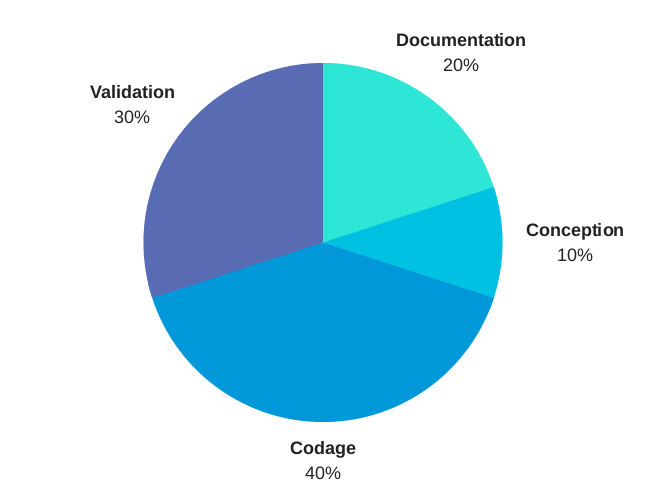
\includegraphics[scale=0.30]{temps_passe.png}
\end{figure}
\newline
Nous avons fait le choix d'accorder une grande partie de notre temps à la validation, car il nous parait fondamentale d'avoir une grande base
de test pour délivrer un produit final de qualité. En revanche, peu de temps a été alloué à la conception, en comparaison à celui dédié à la validation et au codage. \newline \\
Cela n'a pas posé de problème pour l'étape B, et par mimétisme, nous avons
adopter le même plan pour l'étape C. Cependant nous réalisons maintenant que nous aurions peut être du, pour l'étape C,
accorder plus de temps à cette étape de conception, qui nous aurait probablement permis de produire un code plus efficace, et ainsi
de gagner sur le temps de codage. Pour l'étape C, le temps aurait peut être été mieux réparti de cette façon:
\begin{figure}[ht]
\centering
      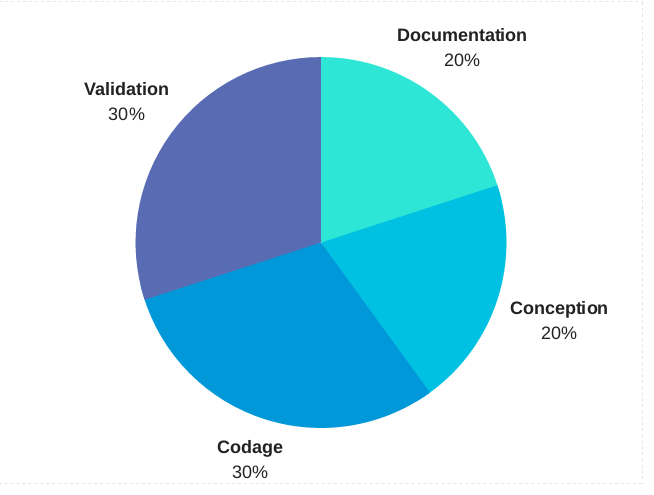
\includegraphics[scale=0.30]{coucou.png}
\end{figure}
\\
Il nous parait alors essentiel, à l'avenir, d'accorder plus d'importance à cette phase de conception, qui pourrait nous faire gagner
du temps sur la phase de codage, tout en améliorant la qualité du produit final.
\\
Concernant l'extension Math, le temps a été réparti de la manière suivante:
\begin{figure}[ht]
\centering
      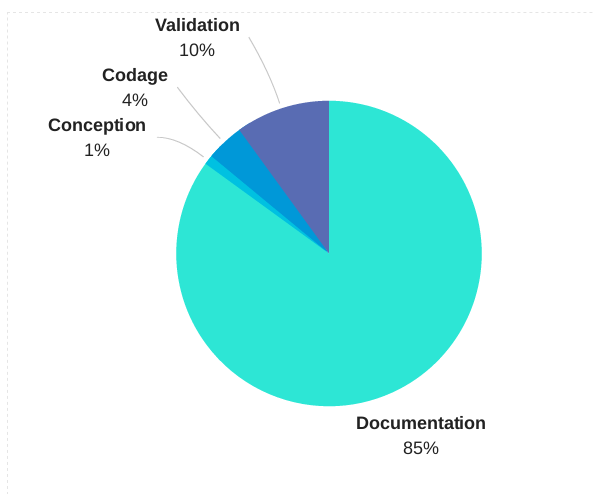
\includegraphics[scale=0.34]{theo.png}
\end{figure}
\newpage
On remarque que la documentation représente la grande majorité du temps. Cela s'explique par la liberté que nous avions concernant
l'extension et par l'absence de consignes et directives à proprement parlé (par opposition au reste du compilateur!). \\
La documentation sur cette partie était périlleuse car, même sur Internet, il a été difficile de trouver les bonnes sources. Il était facile
de rencontrer des algorithmes simples, mais ceux-ci n'étant pas assez précis dans le cadre de notre travail, nous devions fouiner sur les
forums (Stack Overflow), dans des comptes rendus de thèse ou encore dans de gros livres (\textit{Elementary Functions}). La quasi totalité de
la littérature se trouve en anglais, ce qui nous a permis de réaliser une fois de plus l'importance de cette langue dans le milieu
professionnel. \\
\\
Une fois que la période de documentation fût révolue, nous avons développé les algorithmes en Java (car facile à traduire en Déca par la suite).
Cela n'a pas pris longtemps car les algorithmes étaient à notre porté. (La conception au niveau des classes est élémentaire: une class Math
avec quelques constantes en attribut et les méthodes qui vont avec). \\
La deuxième étape la plus chronophage fût la partie de validation, avec l'élaboration de graphiques pour tester la précision des algorithmes
choisis et pour comparer les algorithmes les uns avec les autres.

\newpage
\section{Rétrospective sur les enseignements de ce projet}
Tout au long de ce mois, nous avons pris des décisions en équipe, mais aussi de manière autonome.
Nous pensons que certaines ont été les bonnes, d'autres, avec du recul, nous paraissent maintenant moins judicieuses: ce sont principalement celles liées à l'étape C, avec une mauvaise gestion du temps et des ressources.
\newline
Ainsi, nous avons décidé de classer les enseignements de ce projet en deux catégories : organisationnelles et techniques.
\begin{itemize}
\item Tout d'abord, nous pensons qu'un des plus importants enseignements que nous avons pu tirer de ce projet
porte sur la gestion d'un projet conséquent (un des premiers jusque là!). En effet l'attribution précise des rôles, les réunions
 quotidiennes, le travail quotidien en équipe,
la définition des règles avant un rendu, la mise en place de règles de travail sont des notions auxquelles nous
 n'avions pas pensé la première semaine de ce projet, mais qui nous paraissent maintenant primordiales.
Le maintien d'un cadre de travail agréable pour l'ensemble de l'équipe est aussi primordial à la conception d'un produit final de qualité. Un autre point clé de ce projet à aussi été sa durée. Nous avons appris à tenir notre équipe unie dans l'adversité, et ce sur le long-terme.
\item Puis, bien évidemment, un enseignement technique important du fait de la grande diversité des notions abordés :
antlr4, java, théorie des langages, la génération de code etc...\\
Mais également au niveau de l'utilisation de nouveaux environnements de travail, tel que Maeven, Netbeans, Cobertura pour les tests et une gestion poussée du Git. \\
Concernant la classe Math, elle nous a permis de sensibiliser l'ensemble de l'équipe aux notions d'erreurs machines ce qui est,
d'après nous, essentiel pour un ingénieur en informatique.\\
\end{itemize}

Pour conclure, nous sommes convaincus que le respect des règles et des rôles attribués à chacun nous a permis de travailler
dans un environnement sans conflit ni tension. Malgré quelques mauvaises décisions qui ont impacté la qualité du compilateur, il fut très agréable de travailler au quotidien dans le cadre de ce projet (toujours, modulo le nombre de bugs à résoudre)!



\end{document}
